\documentclass{article}

\usepackage[utf8]{inputenc}
\usepackage[T1]{fontenc}
\usepackage{lipsum}
\usepackage{graphicx}
\usepackage{amsmath}
\usepackage[margin=1in]{geometry}
\usepackage{titlesec}
\usepackage{enumitem}

\titleformat{\section}
{\LARGE\bfseries}{\thesection}{1em}{}

\titleformat{\subsection}
{\Large\bfseries}{\thesection}{1em}{}

\begin{document}
\pagestyle{empty}
\section*{Design model}
\large

\subsection*{Introduzione}
\large
Obiettivi:
\begin{itemize}
    \renewcommand{\labelitemi}{-}
    \itemsep0em
    \item Definire object-oriented analysis e design
    \item Illustrare un esempio relativo
\end{itemize}
Conoscere un linguaggio di programmazione ad oggetti, come Java, è uno step necessario ma non sufficiente per la creazione di un sistema.\ Apprendere come \textit{pensare ad oggetti} sicuramente non rappresenta un passaggio semplice, ma favorisce alla creazione di software robusti, ben progettati e manuntenibili, caratteristiche esterne ed interne che valorizzano al massimo lo sviluppo e l'implementazione di un progetto.\vspace*{14pt}\\
Tutti i passi che richiedono la metamorfosi di un \textit{domain model} ad un \textit{object-oriented model} non sono mai componenti di un procedimento meccanico, poichè, giunti a tale punto, è stata già effettuata un'analisi del problema e dei requisiti essenziali che dovranno essere poi riproposti all'interno della soluzione.\ Per cui si riconosce ciò che il sistema dovrebbe fare, ora occorre progettare un procedimento automatico che compia ogni attività voluta.\vspace*{14pt}\\
Il termine \textit{design} sottolinea una \textit{soluzione concettuale} che rientri appieno nei requisiti, ancora prima di una vera e propria implementazione; per cui conclusi diagrammi comportamentali, come \textit{use case} oppure \textit{activity diagram}, e diagrammi strutturali, come \textit{class diagram}, la fase successiva consiste nella definizione degli oggetti software e al modo in cui essi interagiscono per poter soddisfare tutte le richieste.
\subsection*{Modello decisionale}
\large
Spesso è adottato un modello decisionale ispirato alle specifiche del framework \textit{Unified Process}.\ L'elenco funzionale seguente rappresenta un esempio a cui ispirarsi, una semplificazione, dato che per progetti sempre più complessi e dettagliati il modello potrebbe racchiudere aspetti sempre più specifici e sottili.\vspace*{14pt}\\
Un tipico approccio risulta:
\begin{itemize}
    \renewcommand{\labelitemi}{-}
    \itemsep0em
    \item Definizione dei \textit{casi d'uso}.\ La progettazione di sistemi software nasce dall'esigenza di certi requisiti funzionali, i quali possono essere descritti sintatticamente mediante il \textit{diagramma dei casi d'uso}, rispettando tutte le condizioni del contesto adottato.
    \item Definizione dei \textit{diagrammi di interazione}.\ Il passaggio da una qualsiasi modellazione al \textit{Object-Oriented design}, avviene per formalizzare oggetti software e le loro interazioni.\ Una soluzione spesso adottata consiste nell'uso del \textit{sequence diagram}, capace di illustrare come gli oggetti interagiscono per mezzo di segnali, articolati in molteplici \textit{lifelines}.\ Come da regola del \textit{framework}, un diagramma di interazioni deve essere adeguato per ogni \textit{use case} del punto precedente.
    \item Definizione del \textit{diagramma delle classi}.\ Stabilito il modello che rappresenti una visualizzazione dinamica delle differenti interazioni, potrebbe essere utile ai fini implementativi analizzare un approccio statico mediante singole \textit{classi} che caratterizzino gli oggetti.\ Perciò è adoperato il \textit{diagramma delle classi}, capace di descrivere azioni e attributi inerenti al sistema.
    \item Dividere il sistema in \textit{interface layer} e in \textit{domain layer}.\ Questo step rescinde chiaramente il lato amministratore dal lato client, attribuendo differenti finalità rispetto all'utente che si interfacci con il sistema.\ Le ragioni che spingono tale suddivisione sono relative ad azioni di manutenzione e di modifica al sistema software, in cui lo sviluppatore abbia piena libertà di poter apportare cambiamenti, senza che incidi sull'usufruibilità dell'utente finale.
\end{itemize}
\textit{Esempio}\\
Il \textit{modello decisionale} illustra i passaggi principali che possano indirizzare un'analisi pregressa ad un'implementazione del sistema.\ Di seguito è riportato il procedimento attuato per illustrare graficamente la transizione da \textit{use case} a \textit{sequence diagram}.\vspace*{14pt}\\
Sono formulati cinque step totali, affinchè siano sufficienti per la costruzione del \textit{diagramma delle classi}, illustrando interazioni e caratteristiche dei differenti soggetti.\vspace*{14pt}\\
\textit{Primo step}
\begin{center}
    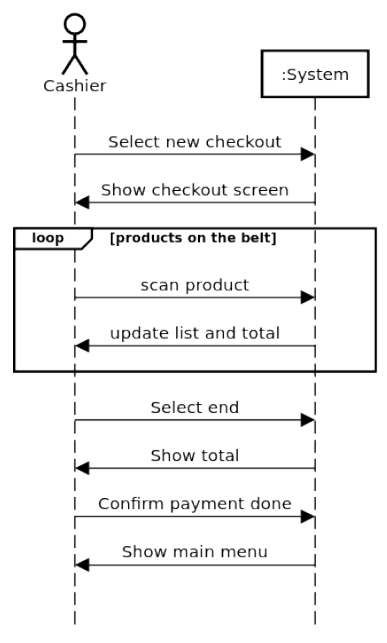
\includegraphics[width=0.4\textwidth]{foto 1.png}
\end{center} 
Il modello raffigura l'attore, in questo caso un \textit{cassiere}, che scannerizza i prodotti mediante l'uso del sistema, per poter individuare il prezzo totale che il \textit{cliente} dovrà poi versare.\vspace*{14pt}\\
Individuato l'obiettivo, si percepisce che il diagramma implementato risulti essere un \textit{sequence diagram}, incentrato nella formalizzazione dell'interazioni che gli attori del \textit{behavioral diagram} si scambiano per mezzo di segnali.\ Per cui, il primo step illustra una porzione del diagramma comportamentale, stabilendo la totalità dei messaggi necessari affinchè sia possibile rispondere alle richieste dei requisiti funzionali.\ Una nota particolare è data dalla presenza di un \textit{loop gate}, ossia al suo interno è ripetuta la medesima operazione fino a quando i prodotti appartenenti alla "spesa" non saranno terminati.\\
Tuttavia un \textit{interation diagram} simile non rispecchia tutte le caratteristiche che possano essere riportate in un seguente \textit{domain model}, perciò occorre inserire ulteriori pattern che analizzino al meglio la struttura delle classi in gioco.\vspace*{14pt}\\
\textit{Secondo step}
\begin{center}
    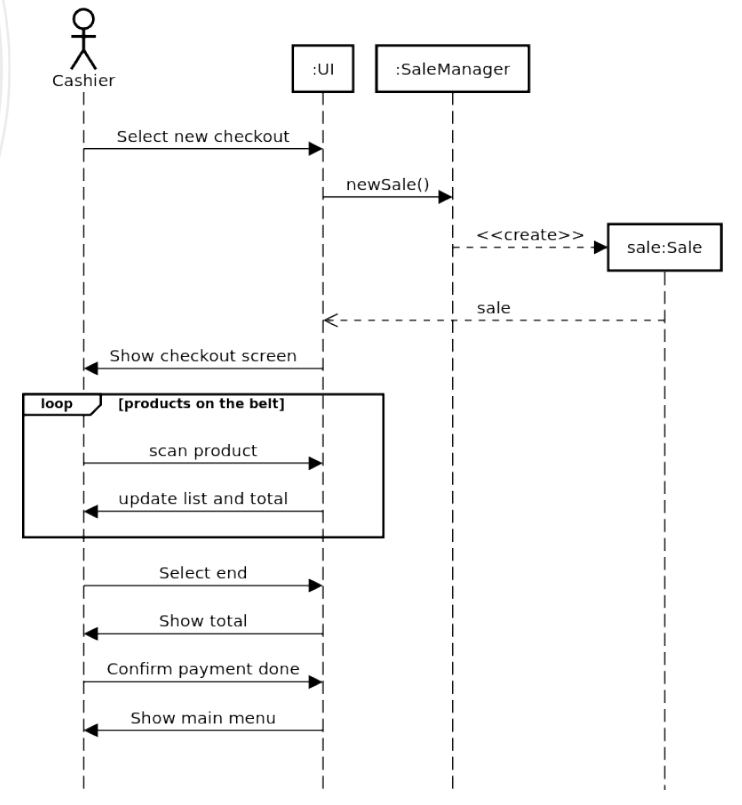
\includegraphics[width=0.8\textwidth]{foto 2.png}
\end{center}
Come da immagine, sono inserite ulteriori istanze.\ Dato che lo scopo nell'uso di un \textit{sequence diagram} consista nell'individuazione di tutte le classi necessarie per un'implementazione, occorre sfruttare al meglio le capacità appartenenti all'\textit{object-oriented design}, capace di distinguere tutte le dipendenze necessarie.\ Il \textit{system} originario è stato distinto in due entità, ossia \textit{UI} e \textit{SaleManager}; quest'ultima azione rispecchia la volontà di suddividere il sistema in un \textit{layer interface}, interpellato dal cassiere, e in un \textit{domain layer}, cioè lato amministratore, colui che provvederà ad inizializzare una nuova vendita, indicata con il nominativo \textit{sale}, ogni volta sia avanzata una richiesta.\vspace*{14pt}\\
\textit{Terzo step}
\begin{center}
    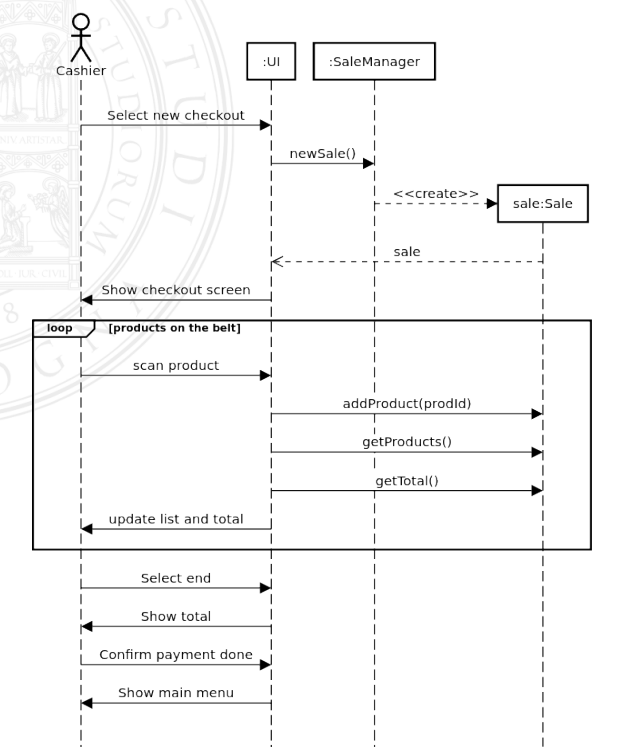
\includegraphics[width=0.8\textwidth]{foto 3.png}
\end{center}
Rispetto alle nuove istanze introdotte, sono inizializzati ulteriori eventi, inerenti alla scannerizzazione di prodotti che compongono la lista.\ Ad ogni scannerizzazione all'interno dell'oggetto \textit{sale} saranno immessi i prodotti in questione, aggiornando il catalogo della "spesa" effettuata e visualizzando ripetitivamente il costo che dovrà essere sostenuto.

\pagebreak
\textit{Quarto step}
\begin{center}
    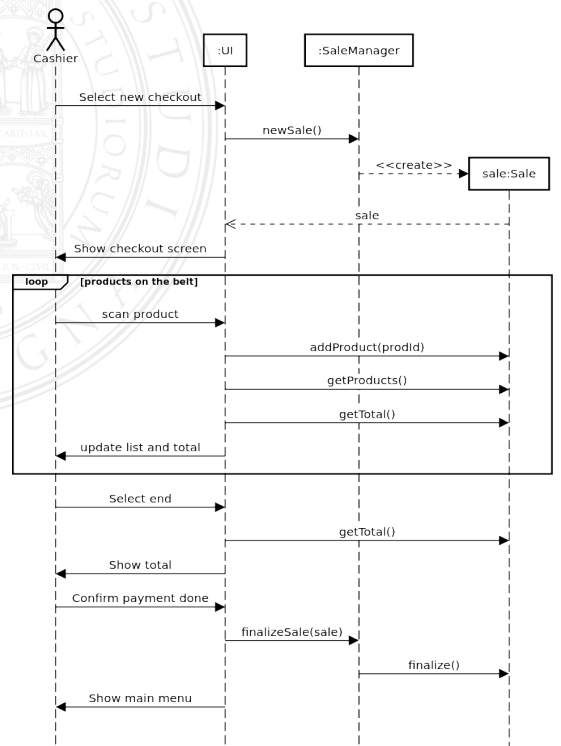
\includegraphics[width=0.8\textwidth]{foto 4.png}
\end{center}\vspace*{14pt}
Concluso il \textit{gate loop}, sarà richiesto dall'attore il totale della spesa.\ Solamente alla conferma del pagamento il cassiere provvederà a interagire con il \textit{SaleManager} per poter finalizzare la vendita da poco avvenuta.\vspace*{14pt}\\
\textit{Quinto step}\\
Il \textit{sequence diagram} riportato, è utilizzato per poter modellare solamente due classi del \textit{domain model}.\ Tuttavia, tramite questo approccio è possibile osservare se l'analisi riportata fino ad ora sia sufficiente o meno per una successiva implementazione.\ E' importante rispettare ogni step proposto, per essere certi della correttezza dei diagrammi modellati e affinchè possano essere aggiunti ulteriori nuovi elementi che rispecchino a pieno ogni requisito funzionale.\vspace*{7pt}
\begin{itemize}
\item[]\begin{minipage}{\textwidth}
  \centering
  \begin{minipage}[t]{0.4\textwidth}
    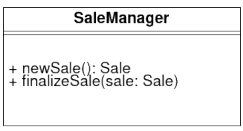
\includegraphics[width=\textwidth]{foto 5.png}
  \end{minipage}
  \begin{minipage}[t]{0.4\textwidth}
    
\includegraphics[width=\textwidth]{foto 6.png}
  \end{minipage}
\end{minipage}
\end{itemize}
\end{document}                  